\documentclass[aspectratio=169]{beamer}
\usepackage{listings}
\usepackage{tabulary}
\usepackage{bm}


\mode<presentation>
{
  %\usetheme{Warsaw}
  % or ...

  \setbeamercovered{transparent}
  % \setbeamercovered{invisible}
  % or whatever (possibly just delete it)
}


\beamertemplatenavigationsymbolsempty

% http://tex.stackexchange.com/questions/160825/modifying-margins-for-one-slide
\newcommand\Wider[2][3em]{%
\makebox[\linewidth][c]{%
  \begin{minipage}{\dimexpr\textwidth+#1\relax}
  \raggedright#2
  \end{minipage}%
  }%
}


\usepackage[english]{babel}
% or whatever

\usepackage[latin1]{inputenc}
% or whatever

% \usepackage{times}
% \usepackage[T1]{fontenc}
% Or whatever. Note that the encoding and the font should match. If T1
% does not look nice, try deleting the line with the fontenc.


% \title[Fortran \& Slide Rules] % (optional, use only with long paper titles)
\title
{Fortran \& Slide Rules}

\subtitle
{Elegant weapons for a more civilized age} % (optional)

\author[Mitton] % (optional, use only with lots of authors)
{kmitton}
% - Use the \inst{?} command only if the authors have different
%   affiliation.

\institute[Yelp] % (optional, but mostly needed)
{
  Yelp
}
% - Use the \inst command only if there are several affiliations.
% - Keep it simple, no one is interested in your street address.

\date[Engineering Learning Group 2015] % (optional)
{Engineering Learning Group / 2015-11-06}

\subject{Talks}
% This is only inserted into the PDF information catalog. Can be left
% out. 




% If you wish to uncover everything in a step-wise fashion, uncomment
% the following command: 

%\beamerdefaultoverlayspecification{<+->}


\begin{document}

\begin{frame}
  \titlepage
\end{frame}

% \begin{frame}{Outline}
%   \tableofcontents
  % You might wish to add the option [pausesections]
% \end{frame}


\section{Fortran}

\subsection{Computers were big}

\begin{frame}[plain]
    % http://www.columbia.edu/cu/computinghistory/704-llnl.jpg
    % 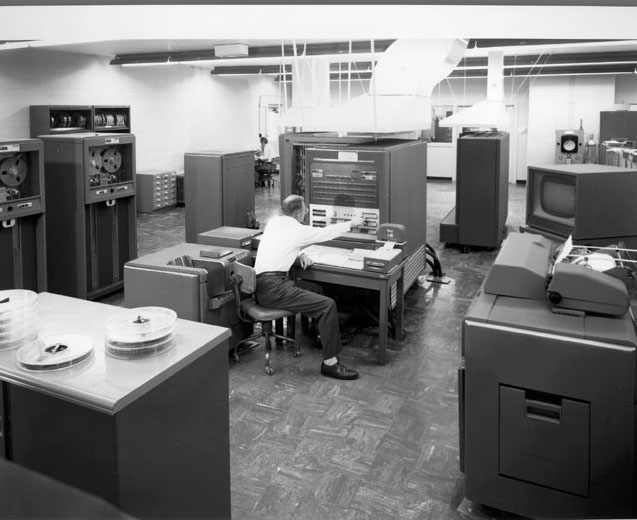
\includegraphics[height=\paperheight]{images/columbia_704-llnl}
    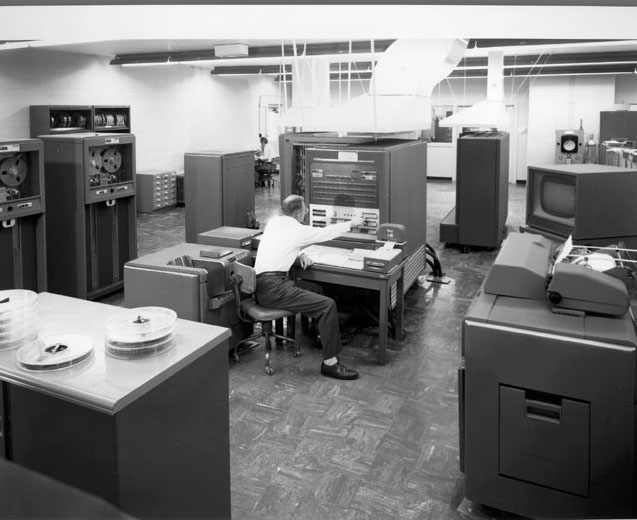
\includegraphics[width=0.8\paperwidth]{images/columbia_704-llnl}
\end{frame}

\begin{frame}[plain]
    % http://www.fortran.com/ibm3.jpg
    \Wider[5em]{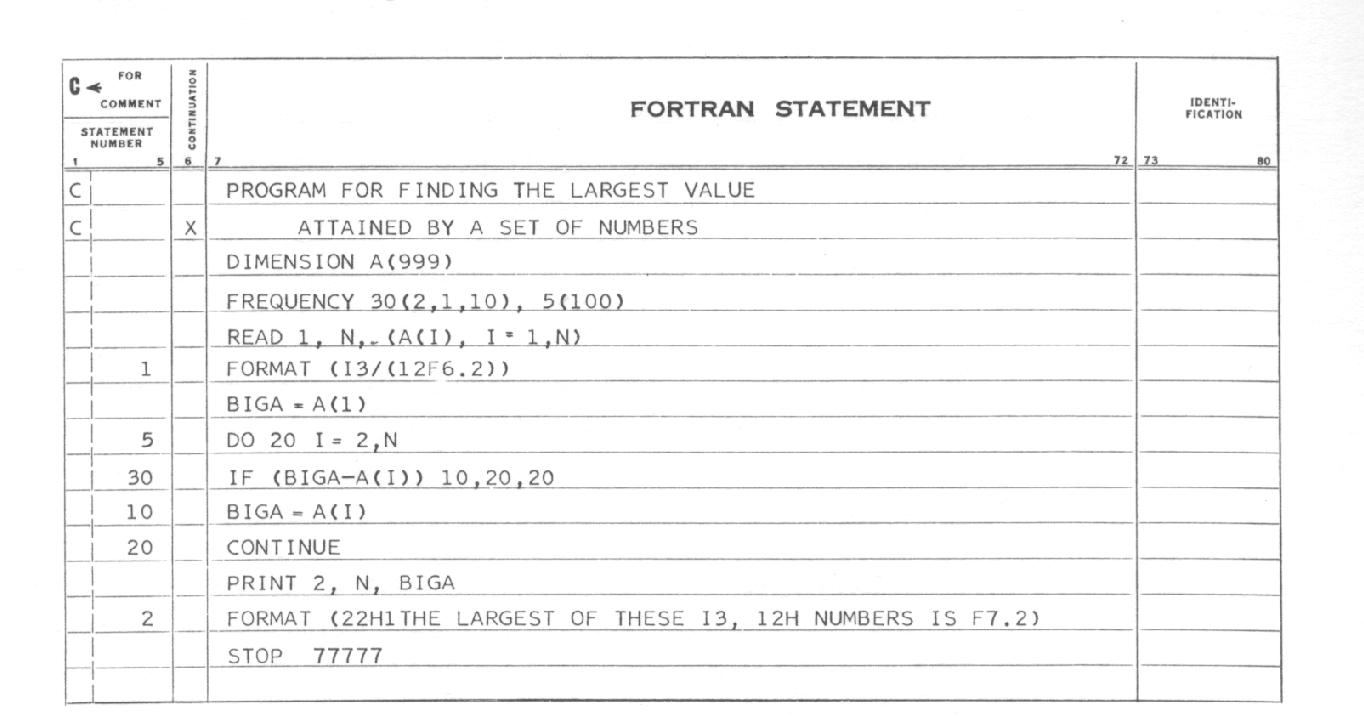
\includegraphics[width=\paperwidth]{images/fortran_ibm3}}
\end{frame}

\begin{frame}[plain]
    % http://commons.wikimedia.org/wiki/File:Punch_card_Fortran_Uni_Stuttgart_(6).jpg
    % https://upload.wikimedia.org/wikipedia/commons/7/76/Punch_card_Fortran_Uni_Stuttgart_%286%29.jpg
    \Wider[5em]{\includegraphics[width=\paperwidth]{images/wikimedia_punchcard}}
\end{frame}


\begin{frame}[fragile]
\lstset{language=Fortran}
    \begin{lstlisting}
C=====================================
C      Computational subroutine 
       subroutine convec(x, y, z, nx, ny) 
       complex*16 x(*), y(*), z(*) 
       integer nx, ny
C      Initialize the output array. 
       do 10 i=1,nx+ny-1
          z(i) = (0.0,0.0) 
 10    continue
       do 30 i=1,nx 
          do 20 j=1,ny
             z(i+j-1) = z(i+j-1) + x(i) * y(j) 
 20       continue
 30    continue 
       return 
       end
    \end{lstlisting}
\end{frame}

\begin{frame}{Significant Fortran versions}
    \begin{tabulary}{\textwidth}{|L|L|L|}
        \hline
        1954-56 & Fortran & 32 statements including arithmetic \texttt{IF}: \newline 
            \texttt{IF (expr) label1, label2, label3} \\
        \hline
        1958 & Fortran II & Subroutines, Functions \\
        \hline
        1961-66 & Fortran IV~/~66 & More data types, modern \texttt{IF} \\
        \hline
        1978 & Fortran 77 & \texttt{CHARACTER} type \\
        \hline
        1991-97 & Fortran 90~/~95 & Free-format source, Modules, \texttt{POINTER}, dynamic memory allocation \\
        \hline
        2003-08 & Fortran 2003~/~2008 & Objects, procedure pointers, I/O enhancements \\
        \hline
        2018 & Fortran 2015 & Tweaks \\
        \hline
    \end{tabulary}
\end{frame}

\begin{frame}{Fortran with legs}
    \begin{tabulary}{\textwidth}{|L|L|}
        \hline
        Basic Linear Algebra Subprograms (BLAS) &
        Level 1: \(\bm{y} \leftarrow \alpha \bm{x} + \bm{y}\) \newline
        Level 2: \(\bm{y} \leftarrow \alpha {A} \bm{x} + \beta \bm{y}\) \newline
        Level 3: \({C} \leftarrow \alpha {AB} + \beta {C}\) \\
        \hline

        Linear Algebra PACKage (LAPACK) &
        Systems of linear equations \newline
        Eigenvalue problems \newline
        Matrix factorizations \\
        \hline

        Scientific computing,
        High Performance Computing &
        Weather simulations, CFD, MATLAB \\
        \hline

    \end{tabulary}
\end{frame}

\begin{frame}{Slide rules}
    \href{http://www.antiquark.com/sliderule/sim/160es/virtual-160-es.html}{antiquark.com Demo Rule}
\end{frame}

\begin{frame}{Slide rule scales}
    \begin{tabulary}{\textwidth}{|L|L|L|}
        \hline
        C, D &
        Standard log scales &
        $*$, $/$ \\
        \hline

        A, B &
        Two-decade log scales &
        $x^2$, $\sqrt{x}$ \\
        \hline

        K &
        Three-decade &
        $x^3$, $x^{1/3}$ \\
        \hline

        CF, DF &
        Folded log scale, runs from $\pi$ to $10\pi$ &
        Useful for results near 10 \\
        \hline

        CI, DI, DIF &
        "Inverted" log scales &
        $1/x$ \\
        \hline

        S, T, ST, SRT &
        Trig scales &
        $\sin, \cos, \tan, \sin^{-1}$ ... \\
        \hline

        L &
        Linear scale &
        $\log_{10}, 10^x$ \\
        \hline

        LLn, $n \in [-3, 3]$ &
        Log-log scales &
        $x^y$ \\
        \hline

        Ln &
        Linear scale &
        $e^x, \ln x$ \\
        \hline

    \end{tabulary}
\end{frame}

\begin{frame}{Designations}
    \begin{tabulary}{\textwidth}{|L|L|}
        \hline
        Mannheim &
        C, D, A, B \\
        \hline

        Polyphase &
        adds K, CI \\
        \hline

        Trig
        Decitrig &
        S, ST, T
        (in tenths of a degree) \\
        \hline

        Log Log &
        LLn \\
        \hline

        Duplex &
        2-sided \\
        \hline

    \end{tabulary}
\end{frame}

\begin{frame}[plain]
    % https://upload.wikimedia.org/wikipedia/commons/f/f7/Circular_slide_rule.JPG
    \Wider[-15em]{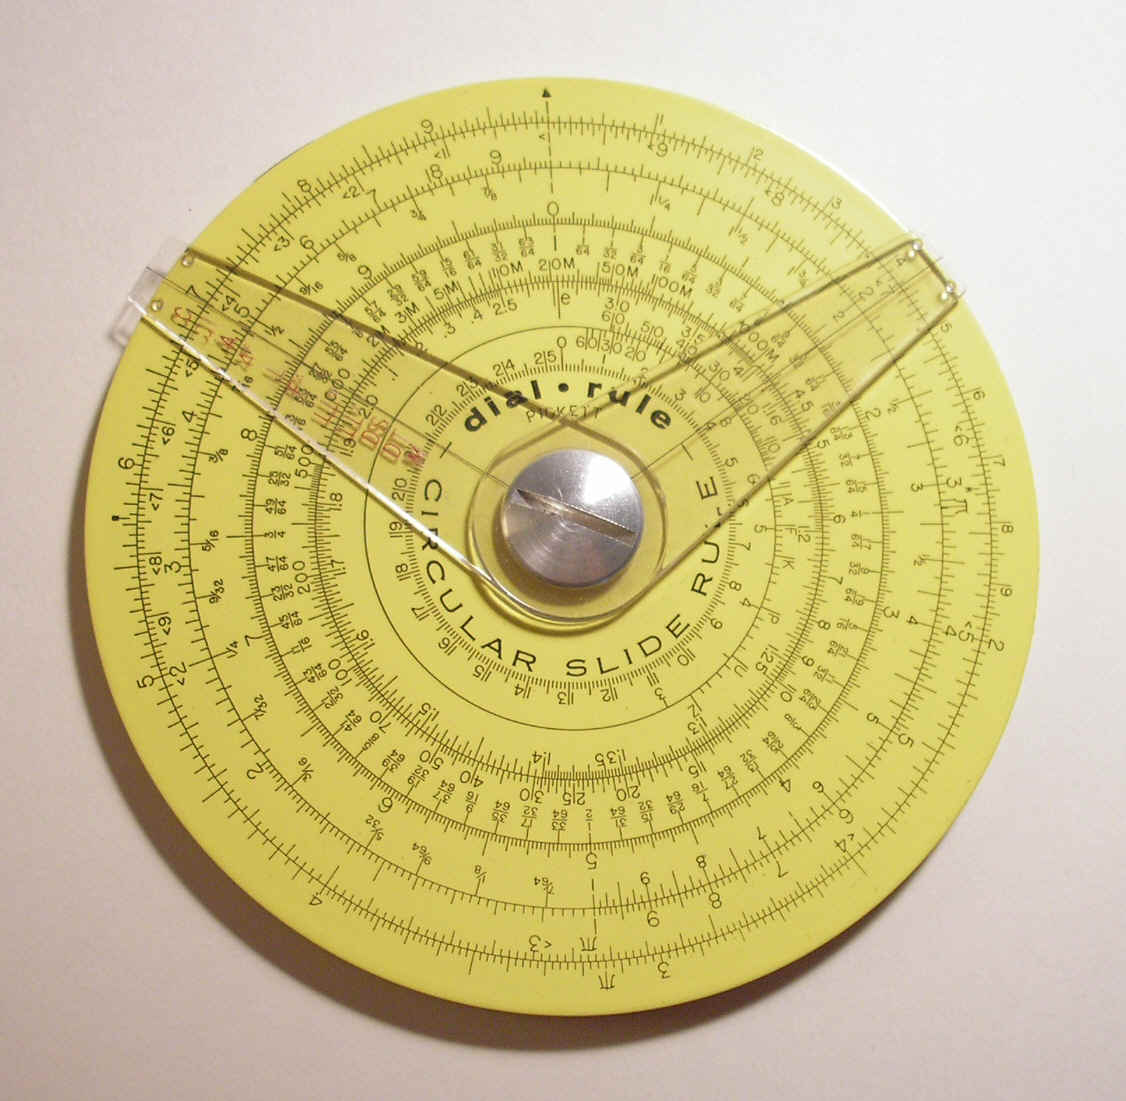
\includegraphics[height=\paperheight]{images/wikimedia_circular_slide_rule}}
\end{frame}

\begin{frame}[plain]
    % http://www.hpmuseum.org/big/fullclse.jpg
    \Wider[5em]{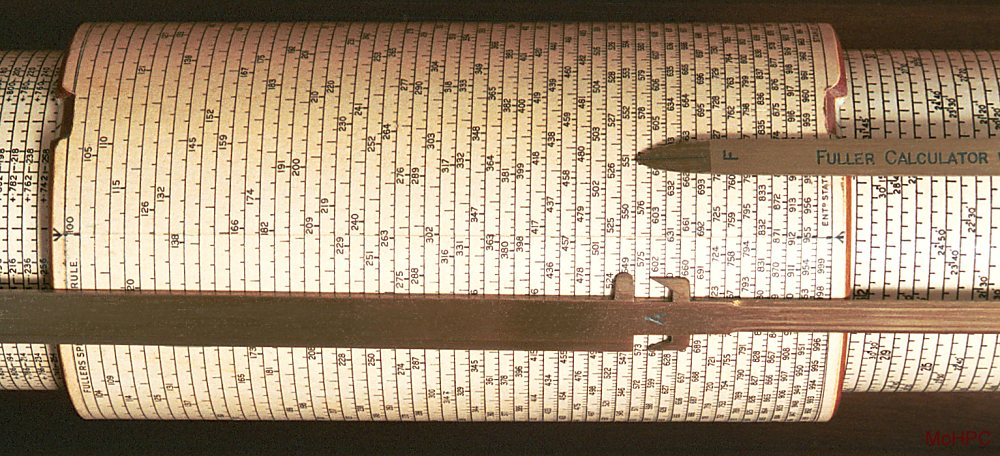
\includegraphics[height=\paperheight]{images/hpmuseum_cylindrical}}
\end{frame}

\begin{frame}{Resources}
    \begin{itemize}
        \item Paper: \href{http://leewm.freeshell.org/origami/}{leewm.freeshell.org/origami}
        \item Web: \href{http://www.antiquark.com/sliderule/sim/}{antiquark.com/sliderule/sim}
        \item iOS: \href{https://itunes.apple.com/us/app/pocket-slide-rule/id421890273?mt=8}
            {Pocket Slide Rule by TestTubeGames}
        \item Android: \href{https://play.google.com/store/apps/details?id=com.timscott.sliderule&hl=en}
            {Slide Rule by Gushiko Studios}
    \end{itemize}
\end{frame}

\end{document}


